% todo: ещё куда-нибудь обязательно надо вхуячить ссылку на ksmt

\section{Датасет}

В своей работе я использовал два датасета с SMT-формулами:

\begin{enumerate}
    \item Бенчмарк\footnote{Набор данных для тестирования корректности или производительности программы.} с SMT-COMP 2023 \cite{smt-comp-2023-benchmarks}.
    \item Формулы, собранные в процессе работы символьного движка USVM.
\end{enumerate}

% todo: здесь ссылка на USVM (Поспелов, 2023)

\subsection{SMT-COMP}

В процессе исследований этот бенчмарк был поделен на три части:

\begin{enumerate}
    \item \texttt{BitVec} --- формулы из логики \texttt{QF\_BV}, обычные формулы с битовыми векторами;
    \item \texttt{SymbEx} --- формулы из логик \texttt{QF\_BV}, \texttt{QF\_ABV}, \texttt{QF\_ABVFP}, \texttt{QF\_AUFBV}, \\ \texttt{QF\_AUFBVFP}, \texttt{QF\_BVFP}, \texttt{QF\_FP}, \texttt{QF\_UF}, \texttt{QF\_UFBV} и \texttt{QF\_UFFP}, которые возникают в процессе работы любого движка для символьного исполнения;
    \item \texttt{QuaFree} --- формулы из всех безкванторных логик, включая \texttt{QF\_LIA}, \texttt{QF\_NRA}, \texttt{QF\_BVFPLRA} и т. д..
\end{enumerate}

Такое разделение обусловлено тем, что для анализа качества хочется смотреть, как модель обучается и какое качество она выдаёт на формулах из разных логик. Однако, к сожалению, большинство логик в данном бенчмарке содержат слишком мало данных, чтобы можно было провести анализ на них, поэтому было принято решение объединить логики в группы по смыслу. Логика \texttt{QF\_BV} была вынесена в отдельную группу, поскольку она является самой многочисленной, а также самой важной на практике. Логики из группы \texttt{SymbEx} были собраны вместе, поскольку моя текущая задача существует в контексте символьного исполнения, поэтому хочется отдельно анализировать способность модели решать подобные формулы. В оставшуюся группу \texttt{QuaFree} попали все безкванторные логики, т. к. хочется также анализировать способность модели решать задачу в некотором общем случае. В дальнейшем каждую группу будем называть датасетом с соответствующим именем.

Формулы с кванторами в данной работе не рассматривались вообще, т. к. они существенно сложнее безкванторных, и их было решено отложить до лучших времён.

Чтобы данные влезли на видеокарту в каждом датасете были оставлены только формулы размером\footnote{Размером формулы считаем количество переменных, констант и операций в ней. Например, размер формулы $(x + y = 5) \vee (z = 3)$ равен 9.} не более 10\,000 и глубиной\footnote{Глубиной формулы считаем максимальную вложенность переменных, констант и операций в ней. Например, глубина формулы $(x + y = 5) \vee (z = 3)$ равна 4.} не более 2\,000. Итоговые параметры построенных датасетов отображены в таблице~\ref{smt-comp-datasets-table}.

\begin{table}[ht]
\begin{center}
\begin{tabular}{r|cccc}
    Датасет & \makecell{Количество \\ формул} & \makecell{Средний \\ размер \\ формулы} & \makecell{Средняя \\ глубина \\ формулы} & \makecell{Доля \\ выполнимых \\ формул} \\
    \hline \hline
    \rule{0pt}{2.5ex}
    \texttt{BitVec} & 33\,797 & 1181.92 & 85.45 & 0.378 \\
    \texttt{SymbEx} & 85\,078 & 669.46 & 49.24 & 0.611 \\
    \texttt{QuaFree} & 123\,396 & 965.16 & 48.71 & 0.622 \\
\end{tabular}
\caption{\label{smt-comp-datasets-table} Параметры датасетов, полученных из данных с SMT-COMP 2023 \cite{smt-comp-2023-benchmarks}.}
\end{center}
\end{table}

\subsection{USVM}

% todo: здесь тоже ссылка на USVM (Поспелов, 2023)

Для проверки возможности применения модели на практике были также вручную собраны датасеты, состоящие из формул, которые возникают в процессе работы символьного движка USVM. Сбор осуществлялся с помощью простого логирования формул, на которых вызывался SMT-решатель. Разные датасеты получались при запуске движка на разных проектах или наборах программ. Подобным образом были собраны три тренировочных и восемнадцать валидационных датасетов.

Такое строгое разделение на тренировочные и валидационные датасеты вдобавок к такому большому количеству вторых обусловлено желанием проверить обобщающую способность модели: хочется, чтобы модель показывала хорошее качество на формулах, возникающих при запуске движка на любых программах; при этом, нет никаких гарантий, что при переходе от одного набора программ к другому распределение, из которого порождаются формулы, изменится несущественно, и качество модели, обученной на данных из другого распределения, упадёт не слишком сильно.

Тренировочные датасеты были собраны на следующих программах:

\begin{enumerate}
    \item \texttt{usvm-test} --- на наборе программ для unit и интеграционного тестирования USVM;
    \item \texttt{the-algorithms} --- на репозитории с реализациями различных теоретических и практических алгоритмов на Java;
    \item \texttt{usvm-core} --- на ядре символьного движка USVM (движок был запущен на самом себе).
\end{enumerate}

Параметры тренировочных датасетов указаны в таблице~\ref{usvm-train-datasets-table}.

\begin{table}[ht]
\begin{center}
\begin{tabular}{r|cccc}
    Датасет & \makecell{Количество \\ формул} & \makecell{Средний \\ размер \\ формулы} & \makecell{Средняя \\ глубина \\ формулы} & \makecell{Доля \\ выполнимых \\ формул} \\
    \hline \hline
    \rule{0pt}{2.5ex}
    \texttt{usvm-test} & 153\,778 & 522.84 & 5.18 & 0.038 \\
    \texttt{the-algorithms} & 181\,633 & 277.03 & 23.94 & 0.066 \\
    \texttt{usvm-core} & 192\,744 & 179.42 & 12.19 & 0.066 \\
\end{tabular}
\caption{\label{usvm-train-datasets-table} Параметры тренировочных датасетов, собранных в процессе работы USVM.}
\end{center}
\end{table}

Валидационные датасеты были собраны при запуске USVM на следующих проектах, написанных на Java и других JVM-языках:

\begin{enumerate}
    \item \texttt{owasp} --- OWASP\footnote{Open Web Application Security Project.}, открытый бенчмарк из программ на Java, на котором оценивают качество инструментов для автоматического поиска уязвимостей в коде \cite{owasp-website};
    \item \texttt{cassandra} --- Apache Cassandra, распределённая NoSQL СУБД\footnote{Система Управления Базами Данных.} \cite{cassandra-website};
    \item \texttt{kafka} --- Apache Kafka, распределённый брокер сообщений \cite{kafka-website};
    \item \texttt{spark-core} --- Apache Spark, система для распределённой обработки данных (модуль ядра) \cite{spark-website};
    \item \texttt{spark-streaming} --- тот же Spark (модуль потоковой обработки данных);
    \item \texttt{utbot-core} --- UnitTestBot, инструмент для автоматической генерации unit-тестов (модуль ядра) \cite{utbot-github};
    \item \texttt{utbot-java} --- тот же UnitTestBot (модуль генерации тестов для Java);
    \item \texttt{utbot-python} --- тот же UnitTestBot (модуль генерации тестов для Python);
    \item \texttt{utbot-js} --- тот же UnitTestBot (модуль генерации тестов для языка JavaScript);
    \item \texttt{utbot-go} --- тот же UnitTestBot (модуль генерации тестов для Go);
    \item \texttt{zookeeper} --- Apache Zookeeper, служба для координации распределённых систем \cite{zookeeper-website};
    \item \texttt{elasticsearch} --- Elasticsearch, встраиваимая система для текстового поиска \cite{elasticsearch-website};
    \item \texttt{hbase} --- Apache HBase, распределённая табличная база данных \cite{hbase-website};
    \item \texttt{guava} --- Google Guava, набор библиотек-расширений для Java \cite{guava-website};
    \item \texttt{hadoop-common} --- Apache Hadoop, экосистема для распределённого хранения и обработки данных (модуль ядра) \cite{hadoop-website};
    \item \texttt{hadoop-hdfs} --- тот же Hadoop (модуль распределённой файловой системы);
    \item \texttt{hadoop-mapreduce} --- тот же Hadoop (модуль для распределённых вычислений в парадигме MapReduce);
    \item \texttt{hadoop-yarn} --- тот же Hadoop (модуль планировщика ресурсов);
\end{enumerate}

Параметры валидационных датасетов указаны в таблице~\ref{usvm-val-datasets-table}.

\begin{table}[ht]
\begin{center}
\begin{tabular}{r|cccc}
    Датасет & \makecell{Количество \\ формул} & \makecell{Средний \\ размер \\ формулы} & \makecell{Средняя \\ глубина \\ формулы} & \makecell{Доля \\ выполнимых \\ формул} \\
    \hline \hline
    \rule{0pt}{2.5ex}
    \texttt{owasp} & 30\,935 & 3169.44 & 27.0 & 0.029 \\
    \texttt{cassandra} & 13\,896 & 164.84 & 11.73 & 0.057 \\
    \texttt{kafka} & 46\,867 & 5103.27 & 18.93 & 0.083 \\
    \texttt{spark-core} & 14\,504 & 5599.33 & 28.0 & 0.061 \\
    \texttt{spark-streaming} & 69\,254 & 1168.64 & 8.31 & 0.057 \\
    \texttt{utbot-core} & 31\,043 & 4570.6 & 28.95 & 0.061 \\
    \texttt{utbot-java} & 12\,492 & 116.4 & 10.71 & 0.045 \\
    \texttt{utbot-python} & 24\,893 & 266.66 & 6.04 & 0.115 \\
    \texttt{utbot-js} & 13\,276 & 2286.54 & 133.8 & 0.062 \\
    \texttt{utbot-go} & 43\,988 & 281.69 & 19.21 & 0.014 \\
    \texttt{zookeeper} & 38\,631 & 1196.51 & 47.23 & 0.046 \\
    \texttt{elasticsearch} & 38\,967 & 388.62 & 19.72 & 0.001 \\
    \texttt{hbase} & 38\,049 & 3513.78 & 90.81 & 0.019 \\
    \texttt{guava} & 56\,607 & 545.98 & 34.99 & 0.014 \\
    \texttt{hadoop-common} & 41\,255 & 419.05 & 10.32 & 0.081 \\
    \texttt{hadoop-hdfs} & 109\,294 & 2795.7 & 210.87 & 0.032 \\
    \texttt{hadoop-mapreduce} & 12\,044 & 1294.2 & 47.17 & 0.011 \\
    \texttt{hadoop-yarn} & 32\,555 & 120.71 & 13.01 & 0.035 \\
\end{tabular}
\caption{\label{usvm-val-datasets-table} Параметры валидационных датасетов, собранных в процессе работы USVM.}
\end{center}
\end{table}

Отмечу, что в валидационных датасетах также отобраны формулы, размер и глубина которых не превышает 10\,000 и 2\,000 соответственно, но, помимо этого, здесь добавилось ещё одно условие: размер должен быть не меньше некоторого значения, которое подбиралось эмпирическим путём отдельно для каждого датасета (и которое можно угадать, если посмотреть на средний столбец в таблице). Поэтому формулы из валидационных датасетов кажутся больше, чем из тренировочных. Это было сделано, чтобы уменьшить объём данных и ускорить вычисления, а также чтобы оценивать качество модели именно на больших формулах, т. к. кажется, что на практике модель должна существенно помогать движку именно в этом случае.

Ещё внимательный читатель может заметить, что во всех датасетах из формул, собранных в процессе работы USVM, есть огромный дисбаланс классов: меньше десяти процентов формул являются выполнимыми. На самом деле, в этом нет ничего неожиданного, потому что в процессе символьного исполнения программы SMT-решателю действительно чаще всего приходится иметь дело с невыполнимыми формулами.

% todo: кажется, тут стоит ещё дописать
% todo: и ещё можно заменить таблицы на ящики с усами

\subsection{Метрики}

% todo: дописать, почему нам нужны такие метрики

% todo: текстовый подход
% \section{Текстовый подход}

\newpage

\section{Подход с использованием GNN}

\subsection{Архитектура нейронной сети для решения задачи}

В качестве основной архитектуры для решения задачи была выбрана некоторая аппроксимация \underline{\hyperref[gnn-architecture]{GNN}}, работающая схожим образом с тем, что было ранее описано в разделе \underline{\hyperref[gnn-for-scheduling-of-smt-solvers]{GNN for Scheduling of SMT Solvers}} \cite{gnn-for-scheduling-paper}. Здесь используется такая же схема передачи GNN-сообщений по данному на вход абстрактно-синтаксическому дереву (AST) формулы, превращённому в ориентированный ациклический граф для простоты вычислений, однако всё это происходит с некоторыми отличиями:

\begin{enumerate}
    \item рёбра проводятся только в направлении от операндов к операторам (см. пример ниже);
    \item обновление эмбеддингов состояний вершин начинается от истоков графа (листьев AST формулы) и производится в порядке топологической сортировки;
    \item передача векторов-сообщений происходит согласно ориентации рёбер (от начала к концу);
    \item вычисление состояния каждой вершины производится только после вычисления состояний всех вершин, от которых она зависит, т. е. всех других вершин, из которых есть ребро в неё;
    \item указанные вычисления для всех вершин делаются за один проход по формуле;
    \item в конце в качестве итогового вектора-представления формулы используется вектор-состояние стока графа (корневой вершины формулы).
\end{enumerate}

Для лучшего понимания, на рис.~\ref{formula-ast-message-flow} изображён пример графа и того, в каком порядке производятся вычисления состояний вершин.

\begin{figure}[ht]
\begin{center}
    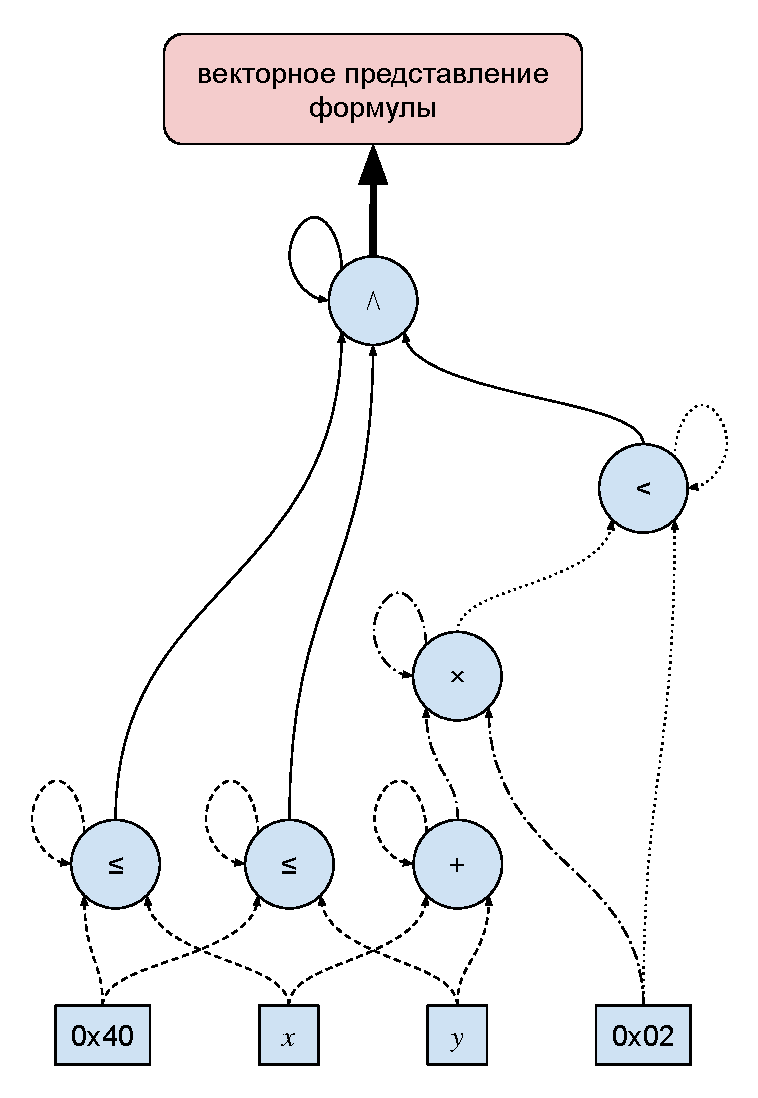
\includegraphics[scale=0.95]{./assets/formula-ast-message-flow.pdf}
    \caption{\label{formula-ast-message-flow} Пример ориентированного ациклического графа, полученного из AST формулы $(\texttt{0x40} \le x) \wedge (\texttt{0x40} \le y) \wedge ((x + y) \times \texttt{0x02} < \texttt{0x02})$ в логике вычислений с восьмибитными векторами. Вершины разбиты по уровням согласно порядку вычислений состояний: снизу истоки (листья) --- с них начинается вычисление, сверху сток (корень) --- его вектор вычисляется последним, и он же считается итоговым вектором-представлением всей формулы. Начертание каждого ребра отражает момент, в который по нему производится передача сообщения: по рёбрам, нарисованным штриховой линией (- - -) передача производится на первом шаге, штрих-пунктирной линией (- $\cdot$ -) --- на втором, пунктирной линией ($\cdot$ $\cdot$ $\cdot$) --- на третьем, а сплошной (\sout{\ \ \ \ \ }) --- на четвёртом. Петли в данном графе обозначают, что для вычисления состояния вершины также используется её начальное состояние (об этом подробнее написано в параграфах про начальные состояния вершин и вычисление их состояний).}
\end{center}
\end{figure}

Описанная выше структура была придумана мной при попытке оптимизировать методы вычислений из статьи \cite{gnn-for-scheduling-paper}, чтобы все нужные состояния можно было посчитать за один проход по AST формулы. Тем не менее, позже, в процессе очередной итерации исследования предметной области, выяснилось, что такая архитектура была придумана ещё в 1997 году, описана в статьях \cite{rvnn-intro-paper} и \cite{rvnn-intro-paper-2} и более известна как рекурсивная нейронная сеть или RvNN\footnote{От англ. \textit{Recursive Neural Network}.}. Авторы указанных статей пытались изобрести подход к обучению моделей для иерархически устроенных данных (рис.~\ref{rvnn-data-tree}), чтобы можно было учитывать и их специфику наряду с тем, как это происходит в свёрточных сетях для данных в виде картинок или в рекуррентных сетях для данных в виде последовательностей. В итоге, было предложено использовать процедуру, похожую на передачу сообщений в GNN, применительно к дереву или ориентированному ациклическому графу, задающим саму иерархию в данных. В статье даже в качестве одного из примеров таких данных рассматриваются логические термы (рис.~\ref{rvnn-term-dag}).

\begin{comment}

\begin{figure}[ht]
\begin{center}

\begin{minipage}{0.45\textwidth}
    \centering
    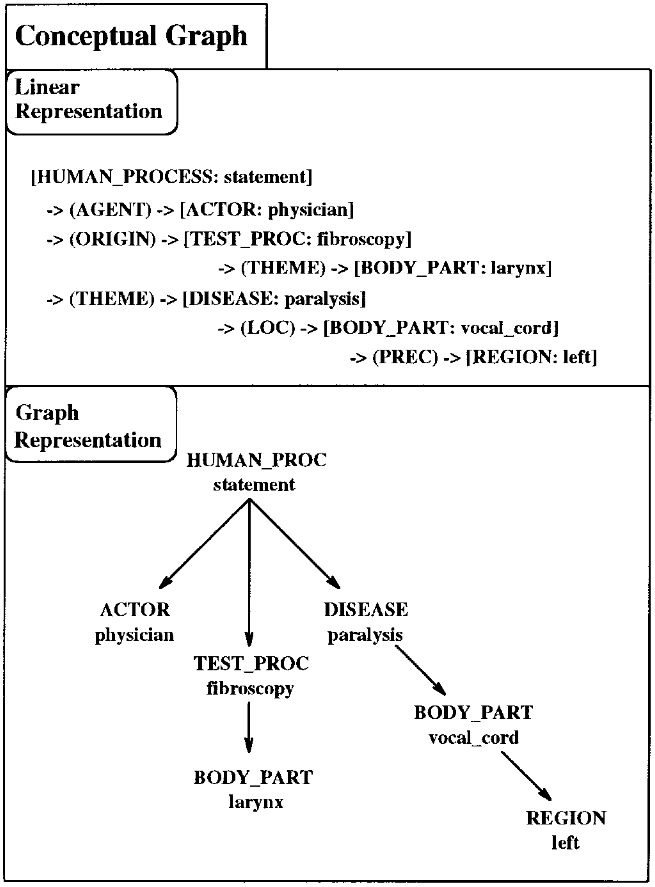
\includegraphics[scale=0.2]{./assets/rvnn-data-tree.png}
    \captionof{figure}{\label{rvnn-data-tree} Пример иерархически устроенных данных: анамнез пациента. Картинка взята из статьи \cite{rvnn-intro-paper}.}
\end{minipage}%
\begin{minipage}{0.45\textwidth}
    \centering
    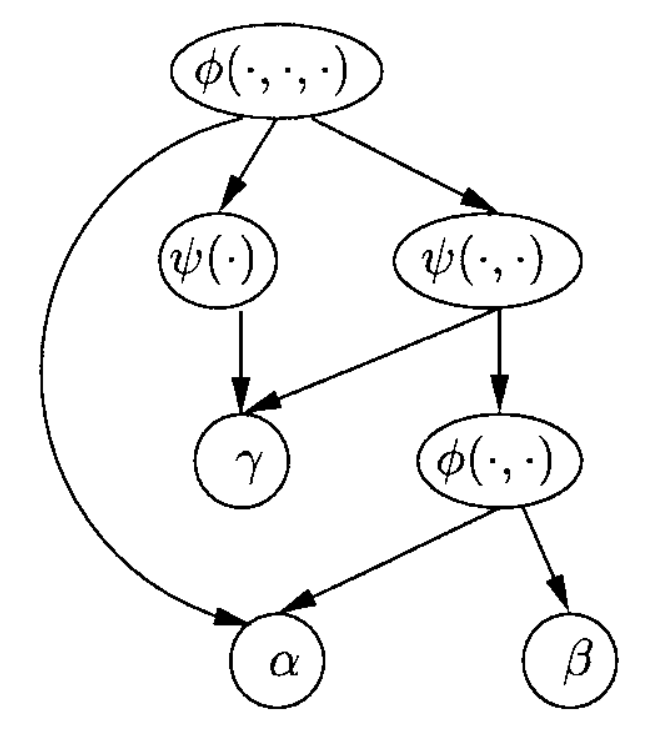
\includegraphics[scale=0.2]{./assets/rvnn-term-dag.png}
    \captionof{figure}{\label{rvnn-term-dag} Пример представления логического терма $\phi(\alpha, \psi(\gamma), \psi(\gamma, \phi(\alpha, \beta)))$ в виде ориентированного ациклического графа. Картинка взята из статьи \cite{rvnn-intro-paper-2}.}
\end{minipage}

\end{center}
\end{figure}

\end{comment}

\begin{figure}[ht]
\begin{center}
    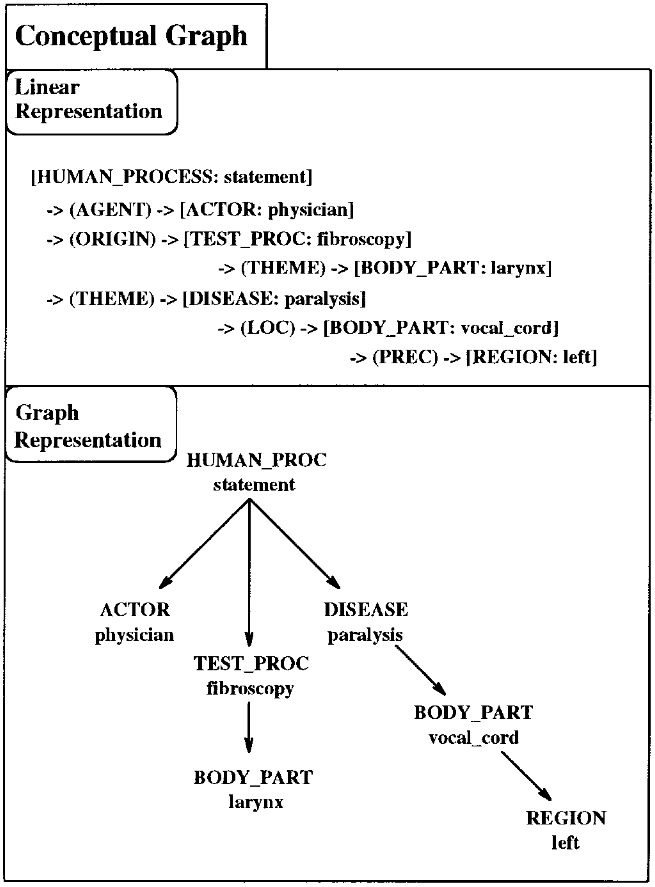
\includegraphics[scale=0.45]{./assets/rvnn-data-tree.png}
    \caption{\label{rvnn-data-tree} Пример иерархически устроенных данных: анамнез пациента. Картинка взята из статьи \cite{rvnn-intro-paper}.}
\end{center}

\begin{center}
    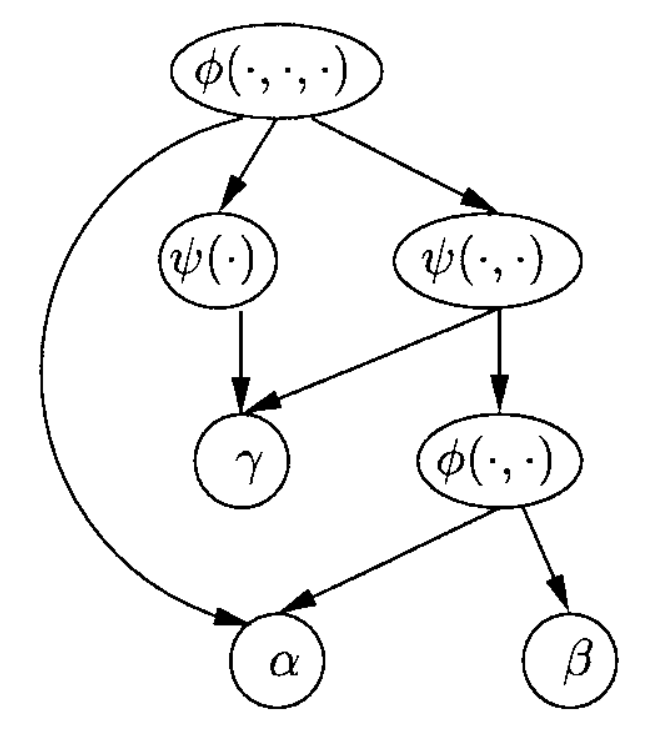
\includegraphics[scale=0.2]{./assets/rvnn-term-dag.png}
    \caption{\label{rvnn-term-dag} Пример представления логического терма $\phi(\alpha, \psi(\gamma), \psi(\gamma, \phi(\alpha, \beta)))$ в виде ориентированного ациклического графа. Картинка взята из статьи \cite{rvnn-intro-paper-2}.}
\end{center}
\end{figure}

Однако с ростом доступных вычислительных мощностей данный подход уступил более обобщённому подходу с использованием GNN и не получил активного дальнейшего развития.

Посчитанный в ходе описанных выше действий вектор-представление графа считается эмбеддингом формулы, который потом можно передать в MLP для предсказания различных параметров формулы, например, её выполнимости. Именно так делается у меня, и ровно так же было предложено делать в статье \cite{rvnn-intro-paper} (рис.~\ref{rvnn-process}).

\begin{figure}[ht]
\begin{center}
    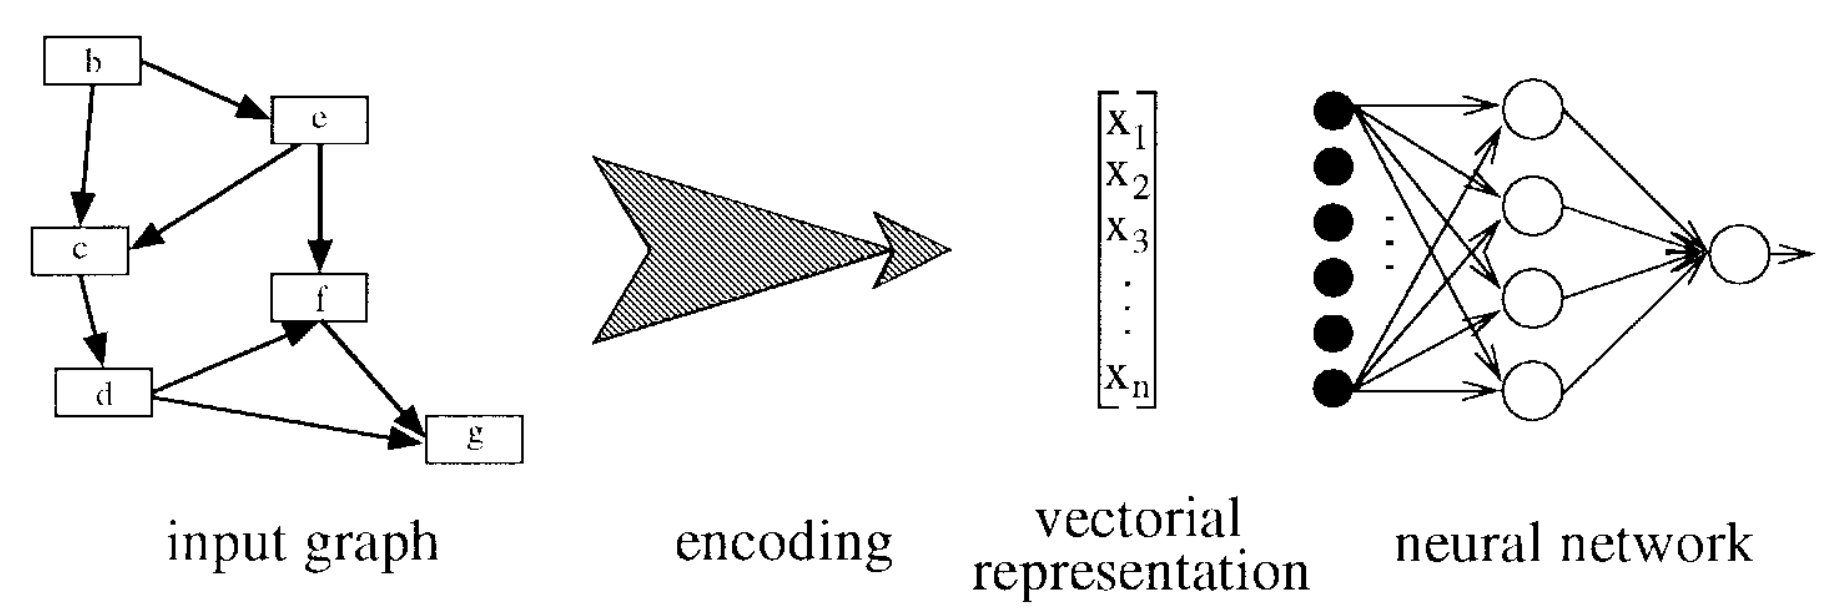
\includegraphics[scale=0.25]{./assets/rvnn-process.png}
    \caption{\label{rvnn-process} Общий подход к решению задачи предсказания произвольных параметров ориентированного ациклического графа. Картинка взята из статьи \cite{rvnn-intro-paper}.}
\end{center}
\end{figure}

\subsection{Начальные состояния вершин}

% * vars and consts

\subsection{Вычисление состояний вершин}

% sage conv
% transformer conv

\subsection{Классификатор и функция потерь}

% \newpage

\section{Эксперименты и результаты}

% todo: тут в основной части можно красивый барплот, а в приложении огромную таблицу

% \newpage

\section{Дальнейшее развитие}

% todo:
% * квантизация и реализация в C++
% * аугментации
% * кванторные формулы
% * представления для переменных/констант
% * двунаправленный message passing
% * Ранжирующий лосс
% * разная ширина эмбеддинга
% * разное количество слоёв MLP
% * пулинг
